% Options for packages loaded elsewhere
\PassOptionsToPackage{unicode}{hyperref}
\PassOptionsToPackage{hyphens}{url}
%
\documentclass[
]{book}
\usepackage{amsmath,amssymb}
\usepackage{lmodern}
\usepackage{iftex}
\ifPDFTeX
  \usepackage[T1]{fontenc}
  \usepackage[utf8]{inputenc}
  \usepackage{textcomp} % provide euro and other symbols
\else % if luatex or xetex
  \usepackage{unicode-math}
  \defaultfontfeatures{Scale=MatchLowercase}
  \defaultfontfeatures[\rmfamily]{Ligatures=TeX,Scale=1}
\fi
% Use upquote if available, for straight quotes in verbatim environments
\IfFileExists{upquote.sty}{\usepackage{upquote}}{}
\IfFileExists{microtype.sty}{% use microtype if available
  \usepackage[]{microtype}
  \UseMicrotypeSet[protrusion]{basicmath} % disable protrusion for tt fonts
}{}
\makeatletter
\@ifundefined{KOMAClassName}{% if non-KOMA class
  \IfFileExists{parskip.sty}{%
    \usepackage{parskip}
  }{% else
    \setlength{\parindent}{0pt}
    \setlength{\parskip}{6pt plus 2pt minus 1pt}}
}{% if KOMA class
  \KOMAoptions{parskip=half}}
\makeatother
\usepackage{xcolor}
\IfFileExists{xurl.sty}{\usepackage{xurl}}{} % add URL line breaks if available
\IfFileExists{bookmark.sty}{\usepackage{bookmark}}{\usepackage{hyperref}}
\hypersetup{
  pdftitle={Proyecto DataViz},
  pdfauthor={Jorge Arteaga y Adriana Palacio},
  hidelinks,
  pdfcreator={LaTeX via pandoc}}
\urlstyle{same} % disable monospaced font for URLs
\usepackage{color}
\usepackage{fancyvrb}
\newcommand{\VerbBar}{|}
\newcommand{\VERB}{\Verb[commandchars=\\\{\}]}
\DefineVerbatimEnvironment{Highlighting}{Verbatim}{commandchars=\\\{\}}
% Add ',fontsize=\small' for more characters per line
\usepackage{framed}
\definecolor{shadecolor}{RGB}{248,248,248}
\newenvironment{Shaded}{\begin{snugshade}}{\end{snugshade}}
\newcommand{\AlertTok}[1]{\textcolor[rgb]{0.94,0.16,0.16}{#1}}
\newcommand{\AnnotationTok}[1]{\textcolor[rgb]{0.56,0.35,0.01}{\textbf{\textit{#1}}}}
\newcommand{\AttributeTok}[1]{\textcolor[rgb]{0.77,0.63,0.00}{#1}}
\newcommand{\BaseNTok}[1]{\textcolor[rgb]{0.00,0.00,0.81}{#1}}
\newcommand{\BuiltInTok}[1]{#1}
\newcommand{\CharTok}[1]{\textcolor[rgb]{0.31,0.60,0.02}{#1}}
\newcommand{\CommentTok}[1]{\textcolor[rgb]{0.56,0.35,0.01}{\textit{#1}}}
\newcommand{\CommentVarTok}[1]{\textcolor[rgb]{0.56,0.35,0.01}{\textbf{\textit{#1}}}}
\newcommand{\ConstantTok}[1]{\textcolor[rgb]{0.00,0.00,0.00}{#1}}
\newcommand{\ControlFlowTok}[1]{\textcolor[rgb]{0.13,0.29,0.53}{\textbf{#1}}}
\newcommand{\DataTypeTok}[1]{\textcolor[rgb]{0.13,0.29,0.53}{#1}}
\newcommand{\DecValTok}[1]{\textcolor[rgb]{0.00,0.00,0.81}{#1}}
\newcommand{\DocumentationTok}[1]{\textcolor[rgb]{0.56,0.35,0.01}{\textbf{\textit{#1}}}}
\newcommand{\ErrorTok}[1]{\textcolor[rgb]{0.64,0.00,0.00}{\textbf{#1}}}
\newcommand{\ExtensionTok}[1]{#1}
\newcommand{\FloatTok}[1]{\textcolor[rgb]{0.00,0.00,0.81}{#1}}
\newcommand{\FunctionTok}[1]{\textcolor[rgb]{0.00,0.00,0.00}{#1}}
\newcommand{\ImportTok}[1]{#1}
\newcommand{\InformationTok}[1]{\textcolor[rgb]{0.56,0.35,0.01}{\textbf{\textit{#1}}}}
\newcommand{\KeywordTok}[1]{\textcolor[rgb]{0.13,0.29,0.53}{\textbf{#1}}}
\newcommand{\NormalTok}[1]{#1}
\newcommand{\OperatorTok}[1]{\textcolor[rgb]{0.81,0.36,0.00}{\textbf{#1}}}
\newcommand{\OtherTok}[1]{\textcolor[rgb]{0.56,0.35,0.01}{#1}}
\newcommand{\PreprocessorTok}[1]{\textcolor[rgb]{0.56,0.35,0.01}{\textit{#1}}}
\newcommand{\RegionMarkerTok}[1]{#1}
\newcommand{\SpecialCharTok}[1]{\textcolor[rgb]{0.00,0.00,0.00}{#1}}
\newcommand{\SpecialStringTok}[1]{\textcolor[rgb]{0.31,0.60,0.02}{#1}}
\newcommand{\StringTok}[1]{\textcolor[rgb]{0.31,0.60,0.02}{#1}}
\newcommand{\VariableTok}[1]{\textcolor[rgb]{0.00,0.00,0.00}{#1}}
\newcommand{\VerbatimStringTok}[1]{\textcolor[rgb]{0.31,0.60,0.02}{#1}}
\newcommand{\WarningTok}[1]{\textcolor[rgb]{0.56,0.35,0.01}{\textbf{\textit{#1}}}}
\usepackage{longtable,booktabs,array}
\usepackage{calc} % for calculating minipage widths
% Correct order of tables after \paragraph or \subparagraph
\usepackage{etoolbox}
\makeatletter
\patchcmd\longtable{\par}{\if@noskipsec\mbox{}\fi\par}{}{}
\makeatother
% Allow footnotes in longtable head/foot
\IfFileExists{footnotehyper.sty}{\usepackage{footnotehyper}}{\usepackage{footnote}}
\makesavenoteenv{longtable}
\usepackage{graphicx}
\makeatletter
\def\maxwidth{\ifdim\Gin@nat@width>\linewidth\linewidth\else\Gin@nat@width\fi}
\def\maxheight{\ifdim\Gin@nat@height>\textheight\textheight\else\Gin@nat@height\fi}
\makeatother
% Scale images if necessary, so that they will not overflow the page
% margins by default, and it is still possible to overwrite the defaults
% using explicit options in \includegraphics[width, height, ...]{}
\setkeys{Gin}{width=\maxwidth,height=\maxheight,keepaspectratio}
% Set default figure placement to htbp
\makeatletter
\def\fps@figure{htbp}
\makeatother
\setlength{\emergencystretch}{3em} % prevent overfull lines
\providecommand{\tightlist}{%
  \setlength{\itemsep}{0pt}\setlength{\parskip}{0pt}}
\setcounter{secnumdepth}{5}
\usepackage{booktabs}
\ifLuaTeX
  \usepackage{selnolig}  % disable illegal ligatures
\fi
\usepackage[]{natbib}
\bibliographystyle{plainnat}

\title{Proyecto DataViz}
\author{Jorge Arteaga y Adriana Palacio}
\date{2021-11-24}

\begin{document}
\maketitle

{
\setcounter{tocdepth}{1}
\tableofcontents
}
\hypertarget{sobre-este-libro}{%
\chapter{Sobre este libro}\label{sobre-este-libro}}

Este libro contiene el detalle del proyecto enfocado a sistemas de información geográfica. Se estará trabajando con un archivo tomado de \emph{Kaggle} en \url{https://www.kaggle.com/dgomonov/data-exploration-on-nyc-airbnb} que contiene información resumida y métricas para Airbnb en la ciudad de Nueva York en 2019.

\hypertarget{paquetes-necesarios}{%
\section{Paquetes Necesarios}\label{paquetes-necesarios}}

Para poder trabajar con datos se hace necesario cargar una serie de librerías.

\begin{enumerate}
\def\labelenumi{\arabic{enumi}.}
\tightlist
\item
  Para el cargue delarchivo csv, utilizaremos el paquete \texttt{readr}.
\item
  Para el manejo de dataframe, utilziaremos el paquete \texttt{dplyr}.
\item
  Para revisión de datos faltantes, utilizaremos los paquetes \texttt{mice} y \texttt{VIM}.
\item
  Para conexión a la base de datos PostgreSQL, utilizaremos el paquete \texttt{RPostgresL}.
\item
  Para poder hacer uso de la API y realizar la conexión a la base de datos con éxito, utilizaremos el paquete \texttt{DBI}
\item
  Para graficar, utilizararemos el paquete \texttt{ggplot2}
\item
  Para visualización en mapas, utilizaremos el paquete \texttt{ggmap}
\end{enumerate}

\begin{Shaded}
\begin{Highlighting}[]
\FunctionTok{library}\NormalTok{(readr)}
\FunctionTok{library}\NormalTok{(dplyr)}
\FunctionTok{library}\NormalTok{(mice)}
\FunctionTok{library}\NormalTok{(VIM)}
\FunctionTok{library}\NormalTok{(DBI)}
\FunctionTok{library}\NormalTok{(RPostgres)}
\FunctionTok{library}\NormalTok{(ggplot2)}
\FunctionTok{library}\NormalTok{(ggmap)}
\end{Highlighting}
\end{Shaded}

\hypertarget{cargue-y-limpieza-de-datos}{%
\chapter{Cargue y Limpieza de Datos}\label{cargue-y-limpieza-de-datos}}

En este capítulo abordaremos el cargue de los datos de AIRBNB de la ciudad de Nueva York en el año 2019.

\hypertarget{carga-de-datos}{%
\section{Carga de datos}\label{carga-de-datos}}

El archivo \texttt{CSV} con el listado de Airbnb de la ciudad de Nueva York para el año 2019 descargado de \emph{Kaggle} se cargará en una base de datos en \texttt{Heroku\ Postgress}. Pero para lograr esto, primero debemos cargar como \texttt{dataframe} el archivo a través de la función \texttt{read.csv()}, agregando la isntrucción \texttt{na\ =\ c("",\ "NA")} para tomar los valores vacíos como datos faltantes \texttt{na}.

\begin{Shaded}
\begin{Highlighting}[]
\NormalTok{airbnb }\OtherTok{\textless{}{-}} \FunctionTok{read.csv}\NormalTok{(}\AttributeTok{file =} \StringTok{"Datasets/AB\_NYC\_2019.csv"}\NormalTok{, }\AttributeTok{na =} \FunctionTok{c}\NormalTok{(}\StringTok{""}\NormalTok{, }\StringTok{"NA"}\NormalTok{))}
\FunctionTok{head}\NormalTok{(airbnb)}
\end{Highlighting}
\end{Shaded}

\begin{verbatim}
##     id                                             name host_id   host_name
## 1 2539               Clean & quiet apt home by the park    2787        John
## 2 2595                            Skylit Midtown Castle    2845    Jennifer
## 3 3647              THE VILLAGE OF HARLEM....NEW YORK !    4632   Elisabeth
## 4 3831                  Cozy Entire Floor of Brownstone    4869 LisaRoxanne
## 5 5022 Entire Apt: Spacious Studio/Loft by central park    7192       Laura
## 6 5099        Large Cozy 1 BR Apartment In Midtown East    7322       Chris
##   neighbourhood_group neighbourhood latitude longitude       room_type price
## 1            Brooklyn    Kensington 40.64749 -73.97237    Private room   149
## 2           Manhattan       Midtown 40.75362 -73.98377 Entire home/apt   225
## 3           Manhattan        Harlem 40.80902 -73.94190    Private room   150
## 4            Brooklyn  Clinton Hill 40.68514 -73.95976 Entire home/apt    89
## 5           Manhattan   East Harlem 40.79851 -73.94399 Entire home/apt    80
## 6           Manhattan   Murray Hill 40.74767 -73.97500 Entire home/apt   200
##   minimum_nights number_of_reviews last_review reviews_per_month
## 1              1                 9  2018-10-19              0.21
## 2              1                45  2019-05-21              0.38
## 3              3                 0        <NA>                NA
## 4              1               270  2019-07-05              4.64
## 5             10                 9  2018-11-19              0.10
## 6              3                74  2019-06-22              0.59
##   calculated_host_listings_count availability_365
## 1                              6              365
## 2                              2              355
## 3                              1              365
## 4                              1              194
## 5                              1                0
## 6                              1              129
\end{verbatim}

Este archivo contiene 48.895 registros y 16 variables para análisis. En la siguiente sección revisaremos si existen datos faltantes en el dataset.

\hypertarget{revisiuxf3n-de-datos-faltantes}{%
\section{Revisión de datos faltantes}\label{revisiuxf3n-de-datos-faltantes}}

Para determinar la existencia de datos faltantes en el dataframe \emph{Airbnb}, primero determinaremos por columna cual es su proporción de datos faltantes contando los valores \texttt{na}.

\begin{Shaded}
\begin{Highlighting}[]
\NormalTok{pMiss }\OtherTok{\textless{}{-}} \ControlFlowTok{function}\NormalTok{(x)\{}\FunctionTok{sum}\NormalTok{(}\FunctionTok{is.na}\NormalTok{(x))}\SpecialCharTok{/}\FunctionTok{length}\NormalTok{(x)}\SpecialCharTok{*}\DecValTok{100}\NormalTok{\}}
\FunctionTok{apply}\NormalTok{(airbnb,}\DecValTok{2}\NormalTok{,pMiss)}
\end{Highlighting}
\end{Shaded}

\begin{verbatim}
##                             id                           name 
##                     0.00000000                     0.03272318 
##                        host_id                      host_name 
##                     0.00000000                     0.04294918 
##            neighbourhood_group                  neighbourhood 
##                     0.00000000                     0.00000000 
##                       latitude                      longitude 
##                     0.00000000                     0.00000000 
##                      room_type                          price 
##                     0.00000000                     0.00000000 
##                 minimum_nights              number_of_reviews 
##                     0.00000000                     0.00000000 
##                    last_review              reviews_per_month 
##                    20.55833930                    20.55833930 
## calculated_host_listings_count               availability_365 
##                     0.00000000                     0.00000000
\end{verbatim}

Tenemos valores faltantes en las colunmnas \texttt{name}, \texttt{host\_name}, \texttt{last\_review} y \texttt{reviews\_per\_month}, sin embargo, solo estas dos últimas estan por encima del umbral seguro (5\%), lo que podría indicarnos a priori que son variables que deben eliminarse porque no aportarán al análisis. Sin embargo, esta es una decisión que debe tomarse con un mayor análisis de estos registros.

Haremos uso de la función \texttt{md.pattern} del paquete \texttt{mice}, que nos brinda visualmente el patron de los datos faltantes, para un mejor entendiemiento de estos.

\begin{Shaded}
\begin{Highlighting}[]
\FunctionTok{md.pattern}\NormalTok{(airbnb, }\AttributeTok{plot =} \ConstantTok{TRUE}\NormalTok{, }\AttributeTok{rotate.names=}\ConstantTok{TRUE}\NormalTok{)}
\end{Highlighting}
\end{Shaded}

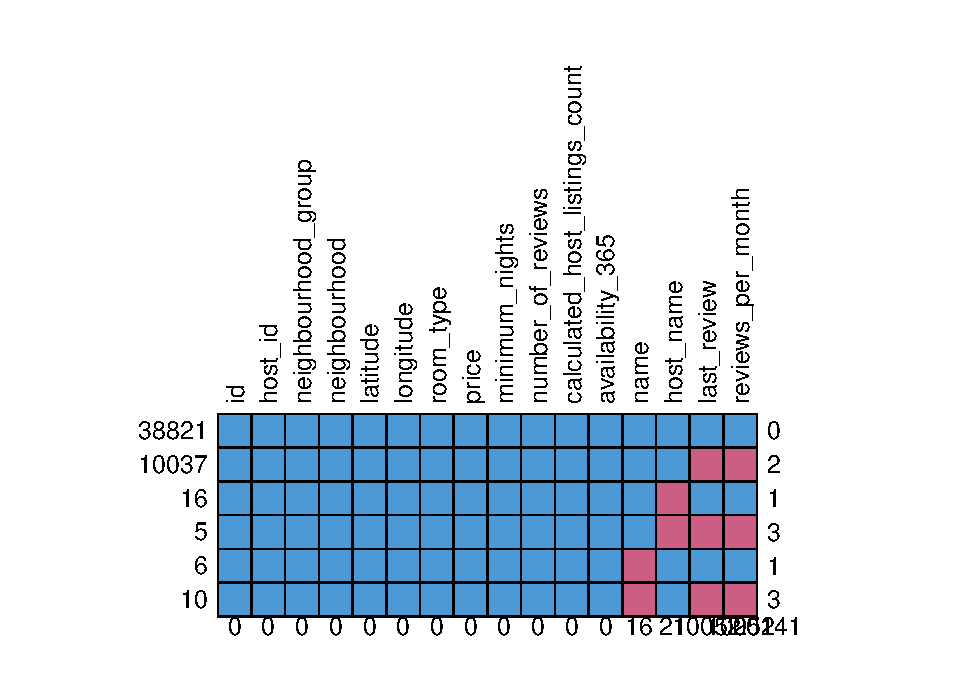
\includegraphics{_main_files/figure-latex/unnamed-chunk-4-1.pdf}

\begin{verbatim}
##       id host_id neighbourhood_group neighbourhood latitude longitude room_type
## 38821  1       1                   1             1        1         1         1
## 10037  1       1                   1             1        1         1         1
## 16     1       1                   1             1        1         1         1
## 5      1       1                   1             1        1         1         1
## 6      1       1                   1             1        1         1         1
## 10     1       1                   1             1        1         1         1
##        0       0                   0             0        0         0         0
##       price minimum_nights number_of_reviews calculated_host_listings_count
## 38821     1              1                 1                              1
## 10037     1              1                 1                              1
## 16        1              1                 1                              1
## 5         1              1                 1                              1
## 6         1              1                 1                              1
## 10        1              1                 1                              1
##           0              0                 0                              0
##       availability_365 name host_name last_review reviews_per_month      
## 38821                1    1         1           1                 1     0
## 10037                1    1         1           0                 0     2
## 16                   1    1         0           1                 1     1
## 5                    1    1         0           0                 0     3
## 6                    1    0         1           1                 1     1
## 10                   1    0         1           0                 0     3
##                      0   16        21       10052             10052 20141
\end{verbatim}

El patrón nos indica que 38.821 registros no tienen datos faltantes, que los datos faltantes se encuentran en las colunmnas \texttt{name}, \texttt{host\_name}, \texttt{last\_review} y \texttt{reviews\_per\_month} (como habíamos encontrado anteriormente), con 16, 21, 10.052 y 10.052 registros, respectivamente. Adicionalmente, el mayor número de registros con datos faltantes (10.037) se encuentran en el patrón que solo contiene \texttt{na} en las columnas \texttt{last\_review} y \texttt{reviews\_per\_month} y solo hay tres filas que contienen más de un valor perdido y de esas solo dos contienen más de dos valores perdidos.

Haciendo uso del paquete \texttt{VIM}, podemos ver la proporción de datos faltantes graficamente. Por cuestión de espacio y mejor visualización del gráfico, trabajaremos con el dataframe solo con la columnas identificadas anteriormente que tienen datos faltantes

\begin{Shaded}
\begin{Highlighting}[]
\NormalTok{airbnb\_columns}\OtherTok{=}\NormalTok{airbnb[,}\FunctionTok{c}\NormalTok{(}\StringTok{"name"}\NormalTok{,}\StringTok{"host\_name"}\NormalTok{,}\StringTok{"last\_review"}\NormalTok{,}\StringTok{"reviews\_per\_month"}\NormalTok{)]}
\FunctionTok{aggr}\NormalTok{(airbnb\_columns, }\AttributeTok{numbers=}\ConstantTok{TRUE}\NormalTok{, }\AttributeTok{sortVars=}\ConstantTok{TRUE}\NormalTok{, }\AttributeTok{labels=}\FunctionTok{names}\NormalTok{(data), }\AttributeTok{cex.axis=}\NormalTok{.}\DecValTok{5}\NormalTok{, }\AttributeTok{gap=}\DecValTok{3}\NormalTok{)}
\end{Highlighting}
\end{Shaded}

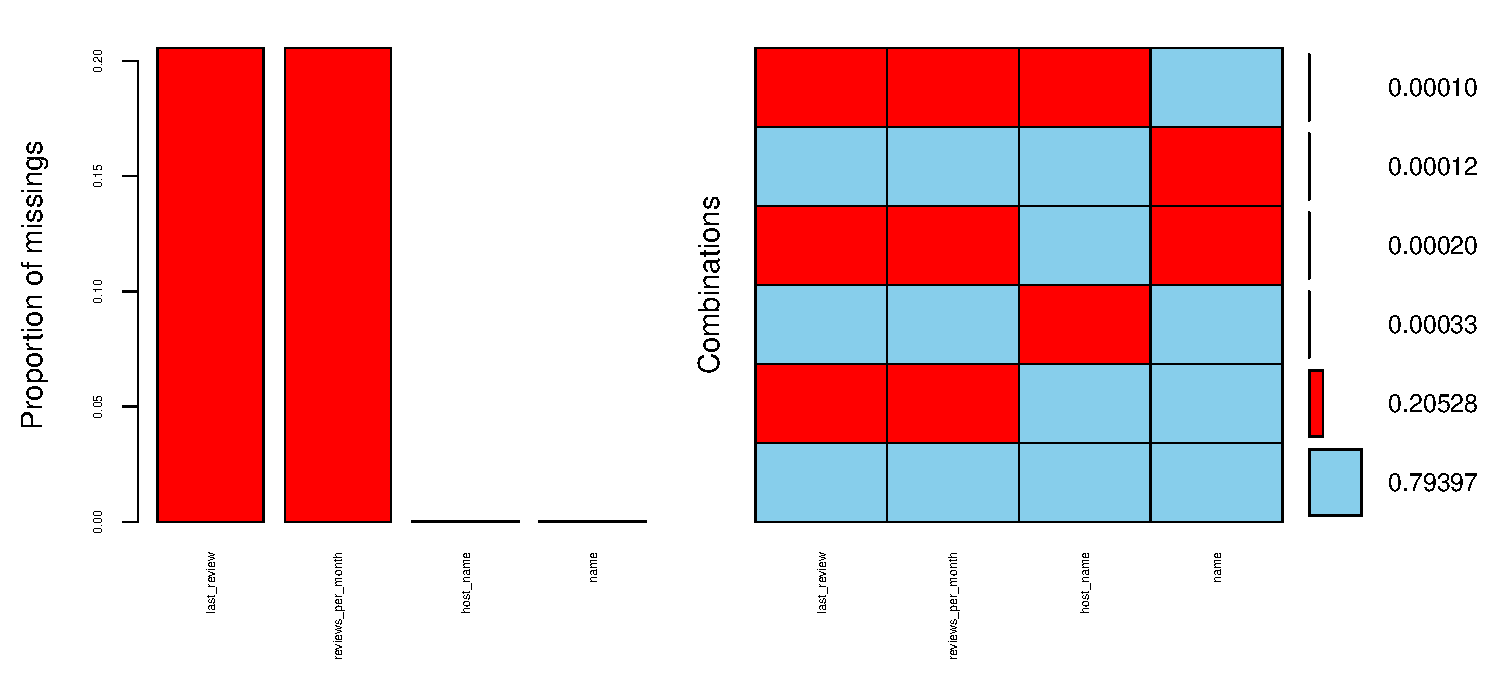
\includegraphics{_main_files/figure-latex/unnamed-chunk-5-1.pdf}

\begin{verbatim}
## 
##  Variables sorted by number of missings: 
##           Variable        Count
##        last_review 0.2055833930
##  reviews_per_month 0.2055833930
##          host_name 0.0004294918
##               name 0.0003272318
\end{verbatim}

El gráfico de barras anterior, nos muestra que las columnas \texttt{last\_review} y \texttt{reviews\_per\_month} representan la mayor proporción de datos faltantes y la proporción para la columnas \texttt{name} y \texttt{host\_name} no es significativa. Este nuevo patrón nos complemente el anterior obtenido con el paquete \texttt{mice}puesto que nos indica adicionalmente que el 79,4\% de los datos no tienen datos perdidos y nos muestra la proporción de filas que tienen un determinado patrón de datos perdidos, por ejemplo, el 20,52\% tienen el patron de datos perdidos solo en las columnas en las columnas \texttt{last\_review} y \texttt{reviews\_per\_month}.

El número de datos perdidos en el dataframe es bastante significativo (20.6\%), sin embargo, al analizar lo que significan las columnas que los tienen, vemos por un lado que para el análisis posterior las columnas \texttt{name} y \texttt{host\_name} no son necesarias y pueden elimminarse.

\begin{Shaded}
\begin{Highlighting}[]
\NormalTok{borrar }\OtherTok{=} \FunctionTok{c}\NormalTok{(}\StringTok{"name"}\NormalTok{, }\StringTok{"host\_name"}\NormalTok{)}
\NormalTok{airbnb }\OtherTok{=}\NormalTok{ airbnb[, }\SpecialCharTok{!}\NormalTok{(}\FunctionTok{names}\NormalTok{(airbnb) }\SpecialCharTok{\%in\%}\NormalTok{ borrar)]}
\FunctionTok{head}\NormalTok{(airbnb)}
\end{Highlighting}
\end{Shaded}

\begin{verbatim}
##     id host_id neighbourhood_group neighbourhood latitude longitude
## 1 2539    2787            Brooklyn    Kensington 40.64749 -73.97237
## 2 2595    2845           Manhattan       Midtown 40.75362 -73.98377
## 3 3647    4632           Manhattan        Harlem 40.80902 -73.94190
## 4 3831    4869            Brooklyn  Clinton Hill 40.68514 -73.95976
## 5 5022    7192           Manhattan   East Harlem 40.79851 -73.94399
## 6 5099    7322           Manhattan   Murray Hill 40.74767 -73.97500
##         room_type price minimum_nights number_of_reviews last_review
## 1    Private room   149              1                 9  2018-10-19
## 2 Entire home/apt   225              1                45  2019-05-21
## 3    Private room   150              3                 0        <NA>
## 4 Entire home/apt    89              1               270  2019-07-05
## 5 Entire home/apt    80             10                 9  2018-11-19
## 6 Entire home/apt   200              3                74  2019-06-22
##   reviews_per_month calculated_host_listings_count availability_365
## 1              0.21                              6              365
## 2              0.38                              2              355
## 3                NA                              1              365
## 4              4.64                              1              194
## 5              0.10                              1                0
## 6              0.59                              1              129
\end{verbatim}

Por otro lado, al analizar los registros faltantes en las columnas \texttt{last\_review} y \texttt{reviews\_per\_month}, encontramos que todos corresponden a aquellos registros donde no existen una evaluación por lo tanto, el manejo de estos datos es simple y se procede de la siguiente manera, se asigna un \texttt{0} en la columna \texttt{reviews\_per\_month} y se elimina la columna \texttt{last\_review} por no tener valor significativo para nuestro análisis posterior.

\begin{Shaded}
\begin{Highlighting}[]
\NormalTok{borrar }\OtherTok{=} \FunctionTok{c}\NormalTok{(}\StringTok{"last\_review"}\NormalTok{)}
\NormalTok{airbnb }\OtherTok{=}\NormalTok{ airbnb[, }\SpecialCharTok{!}\NormalTok{(}\FunctionTok{names}\NormalTok{(airbnb) }\SpecialCharTok{\%in\%}\NormalTok{ borrar)]}

\NormalTok{airbnb }\OtherTok{\textless{}{-}} \FunctionTok{mutate\_at}\NormalTok{(airbnb, }\FunctionTok{c}\NormalTok{(}\StringTok{"reviews\_per\_month"}\NormalTok{), }\SpecialCharTok{\textasciitilde{}}\FunctionTok{replace}\NormalTok{(., }\FunctionTok{is.na}\NormalTok{(.), }\DecValTok{0}\NormalTok{))}
\FunctionTok{head}\NormalTok{(airbnb)}
\end{Highlighting}
\end{Shaded}

\begin{verbatim}
##     id host_id neighbourhood_group neighbourhood latitude longitude
## 1 2539    2787            Brooklyn    Kensington 40.64749 -73.97237
## 2 2595    2845           Manhattan       Midtown 40.75362 -73.98377
## 3 3647    4632           Manhattan        Harlem 40.80902 -73.94190
## 4 3831    4869            Brooklyn  Clinton Hill 40.68514 -73.95976
## 5 5022    7192           Manhattan   East Harlem 40.79851 -73.94399
## 6 5099    7322           Manhattan   Murray Hill 40.74767 -73.97500
##         room_type price minimum_nights number_of_reviews reviews_per_month
## 1    Private room   149              1                 9              0.21
## 2 Entire home/apt   225              1                45              0.38
## 3    Private room   150              3                 0              0.00
## 4 Entire home/apt    89              1               270              4.64
## 5 Entire home/apt    80             10                 9              0.10
## 6 Entire home/apt   200              3                74              0.59
##   calculated_host_listings_count availability_365
## 1                              6              365
## 2                              2              355
## 3                              1              365
## 4                              1              194
## 5                              1                0
## 6                              1              129
\end{verbatim}

En este punto nuestros datos ya no tienen valores faltantes y trabajaremos en adelante con un dataframe de 48.895 y 13 variables.

\begin{Shaded}
\begin{Highlighting}[]
\FunctionTok{apply}\NormalTok{(airbnb,}\DecValTok{2}\NormalTok{,pMiss)}
\end{Highlighting}
\end{Shaded}

\begin{verbatim}
##                             id                        host_id 
##                              0                              0 
##            neighbourhood_group                  neighbourhood 
##                              0                              0 
##                       latitude                      longitude 
##                              0                              0 
##                      room_type                          price 
##                              0                              0 
##                 minimum_nights              number_of_reviews 
##                              0                              0 
##              reviews_per_month calculated_host_listings_count 
##                              0                              0 
##               availability_365 
##                              0
\end{verbatim}

\hypertarget{creaciuxf3n-en-base-de-datos}{%
\section{Creación en base de datos}\label{creaciuxf3n-en-base-de-datos}}

El dataframe sin datos faltantes generado en la sección anterior debe cargarse en una base de datos en \texttt{Heroku\ Postgress}. Para esto primero debemos conectarnos a ella, usando la función \texttt{dbConnect()} con los datos apropiados.

\begin{Shaded}
\begin{Highlighting}[]
\NormalTok{con }\OtherTok{\textless{}{-}} \FunctionTok{dbConnect}\NormalTok{(RPostgres}\SpecialCharTok{::}\FunctionTok{Postgres}\NormalTok{(), }
                \AttributeTok{dbname =} \StringTok{"d41lsl8qgestjf"}\NormalTok{, }
                \AttributeTok{host =} \StringTok{"ec2{-}3{-}229{-}43{-}149.compute{-}1.amazonaws.com"}\NormalTok{, }
                \AttributeTok{port =} \DecValTok{5432}\NormalTok{, }
                \AttributeTok{user =} \StringTok{"uqtxfaqjjcxggw"}\NormalTok{, }
                \AttributeTok{password =} \StringTok{"916d311356954de6a99118d13578bb9d1b47bdc86cb8360a60b9606293bd882d"}\NormalTok{)}
\end{Highlighting}
\end{Shaded}

Una vez tengamos establecida la conexión, insertamos los datos en la tabla \texttt{airbnb}, usando la función \texttt{dbWriteTable()}

\begin{Shaded}
\begin{Highlighting}[]
\FunctionTok{dbWriteTable}\NormalTok{(con, }\StringTok{\textquotesingle{}airbnb\textquotesingle{}}\NormalTok{, airbnb, }\AttributeTok{row.names=}\ConstantTok{FALSE}\NormalTok{, }\AttributeTok{overwrite=}\ConstantTok{TRUE}\NormalTok{)}
\end{Highlighting}
\end{Shaded}

Verifiquemos que podamos leer los datos, através de la función \texttt{dbGetQuery()}

\begin{Shaded}
\begin{Highlighting}[]
\NormalTok{df }\OtherTok{=} \FunctionTok{dbGetQuery}\NormalTok{(con, }\StringTok{"SELECT * FROM airbnb"}\NormalTok{)}
\FunctionTok{summary}\NormalTok{(df)}
\end{Highlighting}
\end{Shaded}

\begin{verbatim}
##        id              host_id          neighbourhood_group neighbourhood     
##  Min.   :    2539   Min.   :     2438   Length:48895        Length:48895      
##  1st Qu.: 9471945   1st Qu.:  7822033   Class :character    Class :character  
##  Median :19677284   Median : 30793816   Mode  :character    Mode  :character  
##  Mean   :19017143   Mean   : 67620011                                         
##  3rd Qu.:29152178   3rd Qu.:107434423                                         
##  Max.   :36487245   Max.   :274321313                                         
##     latitude       longitude       room_type             price        
##  Min.   :40.50   Min.   :-74.24   Length:48895       Min.   :    0.0  
##  1st Qu.:40.69   1st Qu.:-73.98   Class :character   1st Qu.:   69.0  
##  Median :40.72   Median :-73.96   Mode  :character   Median :  106.0  
##  Mean   :40.73   Mean   :-73.95                      Mean   :  152.7  
##  3rd Qu.:40.76   3rd Qu.:-73.94                      3rd Qu.:  175.0  
##  Max.   :40.91   Max.   :-73.71                      Max.   :10000.0  
##  minimum_nights    number_of_reviews reviews_per_month
##  Min.   :   1.00   Min.   :  0.00    Min.   : 0.000   
##  1st Qu.:   1.00   1st Qu.:  1.00    1st Qu.: 0.040   
##  Median :   3.00   Median :  5.00    Median : 0.370   
##  Mean   :   7.03   Mean   : 23.27    Mean   : 1.091   
##  3rd Qu.:   5.00   3rd Qu.: 24.00    3rd Qu.: 1.580   
##  Max.   :1250.00   Max.   :629.00    Max.   :58.500   
##  calculated_host_listings_count availability_365
##  Min.   :  1.000                Min.   :  0.0   
##  1st Qu.:  1.000                1st Qu.:  0.0   
##  Median :  1.000                Median : 45.0   
##  Mean   :  7.144                Mean   :112.8   
##  3rd Qu.:  2.000                3rd Qu.:227.0   
##  Max.   :327.000                Max.   :365.0
\end{verbatim}

\hypertarget{anuxe1lisis-exploratorio-de-los-datos}{%
\chapter{Análisis Exploratorio de los datos}\label{anuxe1lisis-exploratorio-de-los-datos}}

En este capítulo abordaremos el análisis exploratorio de los dato \emph{EDA} para el listado de Airbnb de la ciudad de Nueva York en el año 2019.

\hypertarget{resumen-de-los-datos}{%
\section*{Resumen de los datos}\label{resumen-de-los-datos}}
\addcontentsline{toc}{section}{Resumen de los datos}

Empezamos el análisis exploratorio de nuestros datos con las estadísticas de resumen, haciendo uso de la función \texttt{summary} para los datos contenidos en la tabla \texttt{airbnb} de nuestra base de datos en \texttt{Heroku}

\begin{Shaded}
\begin{Highlighting}[]
\NormalTok{con }\OtherTok{\textless{}{-}} \FunctionTok{dbConnect}\NormalTok{(RPostgres}\SpecialCharTok{::}\FunctionTok{Postgres}\NormalTok{(), }
                \AttributeTok{dbname =} \StringTok{"d41lsl8qgestjf"}\NormalTok{, }
                \AttributeTok{host =} \StringTok{"ec2{-}3{-}229{-}43{-}149.compute{-}1.amazonaws.com"}\NormalTok{, }
                \AttributeTok{port =} \DecValTok{5432}\NormalTok{, }
                \AttributeTok{user =} \StringTok{"uqtxfaqjjcxggw"}\NormalTok{, }
                \AttributeTok{password =} \StringTok{"916d311356954de6a99118d13578bb9d1b47bdc86cb8360a60b9606293bd882d"}\NormalTok{)}

\NormalTok{df }\OtherTok{=} \FunctionTok{dbGetQuery}\NormalTok{(con, }\StringTok{"SELECT * FROM airbnb"}\NormalTok{)}
\FunctionTok{summary}\NormalTok{(df)}
\end{Highlighting}
\end{Shaded}

\begin{verbatim}
##        id              host_id          neighbourhood_group neighbourhood     
##  Min.   :    2539   Min.   :     2438   Length:48895        Length:48895      
##  1st Qu.: 9471945   1st Qu.:  7822033   Class :character    Class :character  
##  Median :19677284   Median : 30793816   Mode  :character    Mode  :character  
##  Mean   :19017143   Mean   : 67620011                                         
##  3rd Qu.:29152178   3rd Qu.:107434423                                         
##  Max.   :36487245   Max.   :274321313                                         
##     latitude       longitude       room_type             price        
##  Min.   :40.50   Min.   :-74.24   Length:48895       Min.   :    0.0  
##  1st Qu.:40.69   1st Qu.:-73.98   Class :character   1st Qu.:   69.0  
##  Median :40.72   Median :-73.96   Mode  :character   Median :  106.0  
##  Mean   :40.73   Mean   :-73.95                      Mean   :  152.7  
##  3rd Qu.:40.76   3rd Qu.:-73.94                      3rd Qu.:  175.0  
##  Max.   :40.91   Max.   :-73.71                      Max.   :10000.0  
##  minimum_nights    number_of_reviews reviews_per_month
##  Min.   :   1.00   Min.   :  0.00    Min.   : 0.000   
##  1st Qu.:   1.00   1st Qu.:  1.00    1st Qu.: 0.040   
##  Median :   3.00   Median :  5.00    Median : 0.370   
##  Mean   :   7.03   Mean   : 23.27    Mean   : 1.091   
##  3rd Qu.:   5.00   3rd Qu.: 24.00    3rd Qu.: 1.580   
##  Max.   :1250.00   Max.   :629.00    Max.   :58.500   
##  calculated_host_listings_count availability_365
##  Min.   :  1.000                Min.   :  0.0   
##  1st Qu.:  1.000                1st Qu.:  0.0   
##  Median :  1.000                Median : 45.0   
##  Mean   :  7.144                Mean   :112.8   
##  3rd Qu.:  2.000                3rd Qu.:227.0   
##  Max.   :327.000                Max.   :365.0
\end{verbatim}

De las columnas de nuestro dataframe, podemos decir por ejemplo que el precio de una noche de los airbnb oscila entre 0 y 10.000 dólares con un promedio de 152.7 dólares, más adelante revisaremos si un precio diario de 10.000 dólares es o no un dato atípico. Adicionalmente, los alojamientos se pueden reservar desde 1 noche sin embargo hay algunos cuyas noches mínimas son de 1.250, alrededor de 3.5 años, esto también es un candidato a dato atípico que será revisado en la siguente sección. Por otro lado, existen anfitriones que tienen hasta 327 alojamientos en la región.

A pesar, que las columnas \texttt{id}, \texttt{host\_id}, \texttt{latitude} y \texttt{longitude} son numéricas, no son relevante las métricas de minimo, máximo, media y cuartiles.

Evaluando los valores que pueden tomar las variables categóricas usando la función \texttt{unique}, encontramos que los tipos de alojamiento disponibles son: Habitaciones privadas (``Private room''), Apartamentos Completos (``Entire home/apt'') o Habitaciones compartidas (``Shared room'') y tenemos grupos de vencindarios como Brooklyn, Manhattan, Qeens, Staten Island y Bronx y en total 221 vecindarios disponibles para alojamiento.

\begin{Shaded}
\begin{Highlighting}[]
\FunctionTok{unique}\NormalTok{(df}\SpecialCharTok{$}\NormalTok{room\_type)}
\end{Highlighting}
\end{Shaded}

\begin{verbatim}
## [1] "Private room"    "Entire home/apt" "Shared room"
\end{verbatim}

\begin{Shaded}
\begin{Highlighting}[]
\FunctionTok{unique}\NormalTok{(df}\SpecialCharTok{$}\NormalTok{neighbourhood\_group)}
\end{Highlighting}
\end{Shaded}

\begin{verbatim}
## [1] "Brooklyn"      "Manhattan"     "Queens"        "Staten Island"
## [5] "Bronx"
\end{verbatim}

\begin{Shaded}
\begin{Highlighting}[]
\FunctionTok{length}\NormalTok{(}\FunctionTok{unique}\NormalTok{(df}\SpecialCharTok{$}\NormalTok{neighbourhood))}
\end{Highlighting}
\end{Shaded}

\begin{verbatim}
## [1] 221
\end{verbatim}

\hypertarget{datos-atuxedpicos}{%
\section*{Datos Atípicos}\label{datos-atuxedpicos}}
\addcontentsline{toc}{section}{Datos Atípicos}

Tenemos sospechas que existen datos atípicos en las columnas \texttt{price} y `minimum\_nights. Al analizar los histogramas y boxplots encontramos que estos abarcan la mayor parte del rango de las variables.

\begin{Shaded}
\begin{Highlighting}[]
\FunctionTok{par}\NormalTok{(}\AttributeTok{mfrow =} \FunctionTok{c}\NormalTok{(}\DecValTok{1}\NormalTok{, }\DecValTok{2}\NormalTok{))}

\FunctionTok{ggplot}\NormalTok{(df) }\SpecialCharTok{+}
  \FunctionTok{aes}\NormalTok{(}\AttributeTok{x =}\NormalTok{ price) }\SpecialCharTok{+}
  \FunctionTok{geom\_histogram}\NormalTok{(}\AttributeTok{fill =} \StringTok{"blue"}\NormalTok{) }\SpecialCharTok{+}
  \FunctionTok{theme\_minimal}\NormalTok{()}
\end{Highlighting}
\end{Shaded}

\begin{verbatim}
## `stat_bin()` using `bins = 30`. Pick better value with `binwidth`.
\end{verbatim}

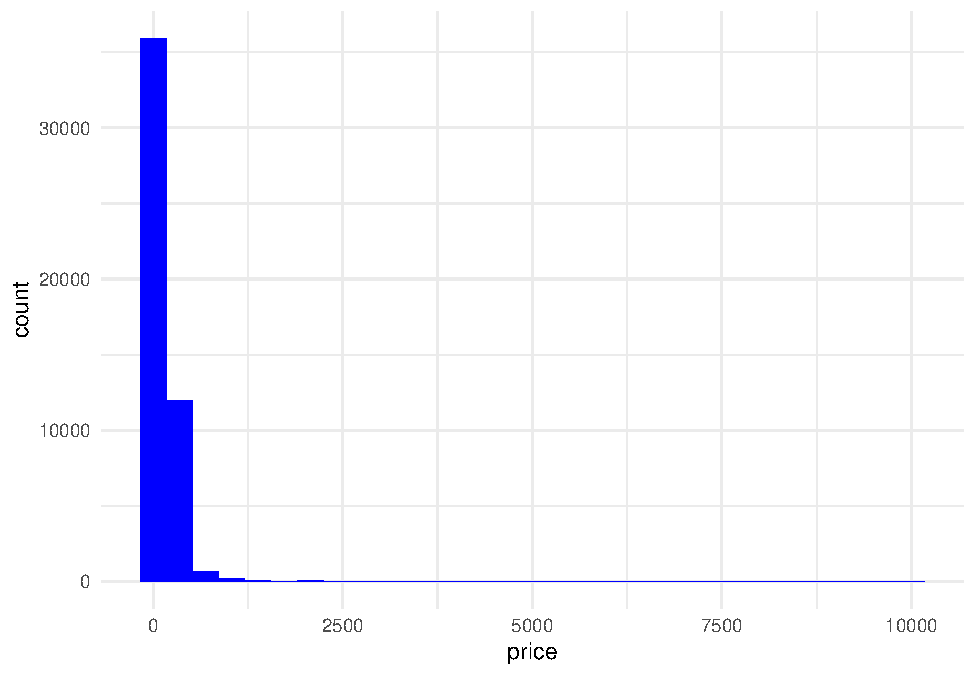
\includegraphics{_main_files/figure-latex/unnamed-chunk-14-1.pdf}

\begin{Shaded}
\begin{Highlighting}[]
\FunctionTok{ggplot}\NormalTok{(df) }\SpecialCharTok{+}
  \FunctionTok{aes}\NormalTok{(}\AttributeTok{x =}\NormalTok{ minimum\_nights) }\SpecialCharTok{+}
  \FunctionTok{geom\_histogram}\NormalTok{(}\AttributeTok{fill =} \StringTok{"red"}\NormalTok{) }\SpecialCharTok{+}
  \FunctionTok{theme\_minimal}\NormalTok{()}
\end{Highlighting}
\end{Shaded}

\begin{verbatim}
## `stat_bin()` using `bins = 30`. Pick better value with `binwidth`.
\end{verbatim}

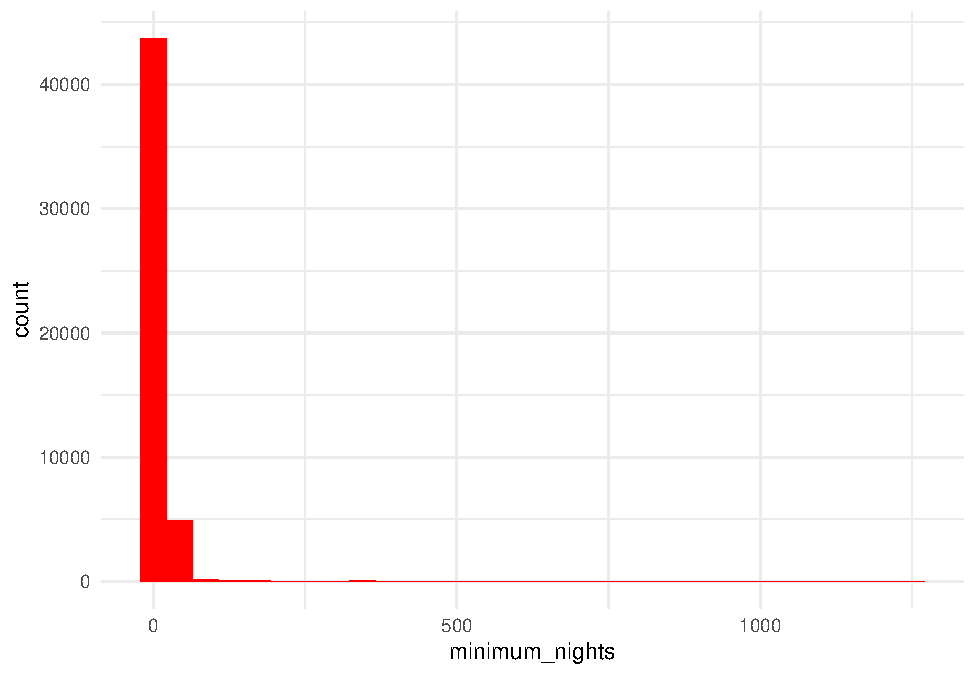
\includegraphics{_main_files/figure-latex/unnamed-chunk-14-2.pdf}

\begin{Shaded}
\begin{Highlighting}[]
\FunctionTok{ggplot}\NormalTok{(df) }\SpecialCharTok{+}
  \FunctionTok{aes}\NormalTok{(}\AttributeTok{x =} \StringTok{""}\NormalTok{, }\AttributeTok{y =}\NormalTok{ price) }\SpecialCharTok{+}
  \FunctionTok{geom\_boxplot}\NormalTok{(}\AttributeTok{fill =} \StringTok{"blue"}\NormalTok{) }\SpecialCharTok{+}
  \FunctionTok{theme\_minimal}\NormalTok{()}
\end{Highlighting}
\end{Shaded}

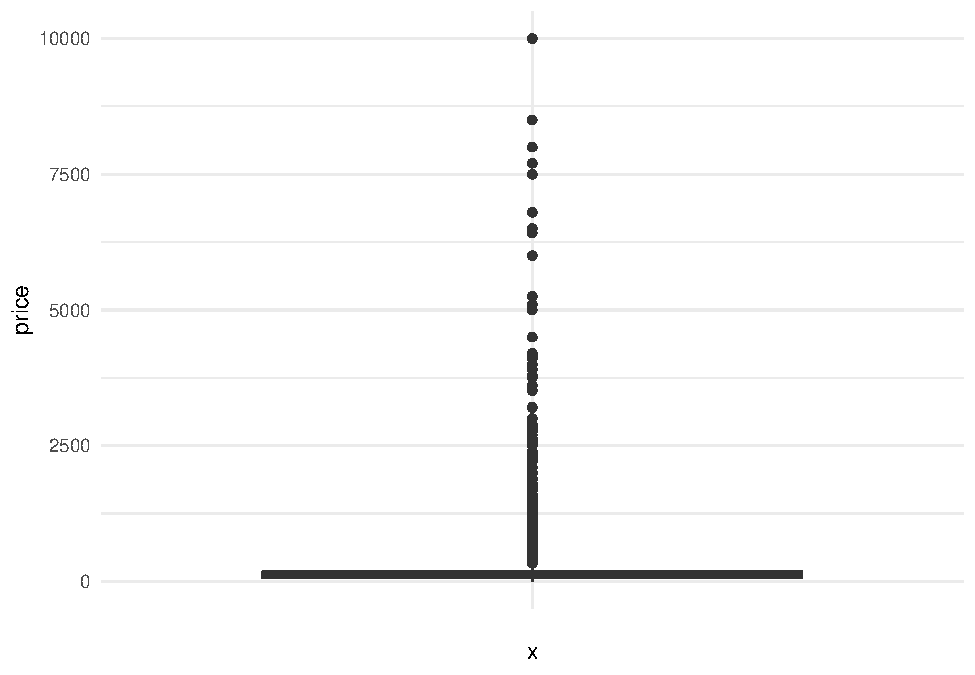
\includegraphics{_main_files/figure-latex/unnamed-chunk-14-3.pdf}

\begin{Shaded}
\begin{Highlighting}[]
\FunctionTok{ggplot}\NormalTok{(df) }\SpecialCharTok{+}
  \FunctionTok{aes}\NormalTok{(}\AttributeTok{x =} \StringTok{""}\NormalTok{, }\AttributeTok{y =}\NormalTok{ minimum\_nights) }\SpecialCharTok{+}
  \FunctionTok{geom\_boxplot}\NormalTok{(}\AttributeTok{fill =} \StringTok{"red"}\NormalTok{) }\SpecialCharTok{+}
  \FunctionTok{theme\_minimal}\NormalTok{()}
\end{Highlighting}
\end{Shaded}

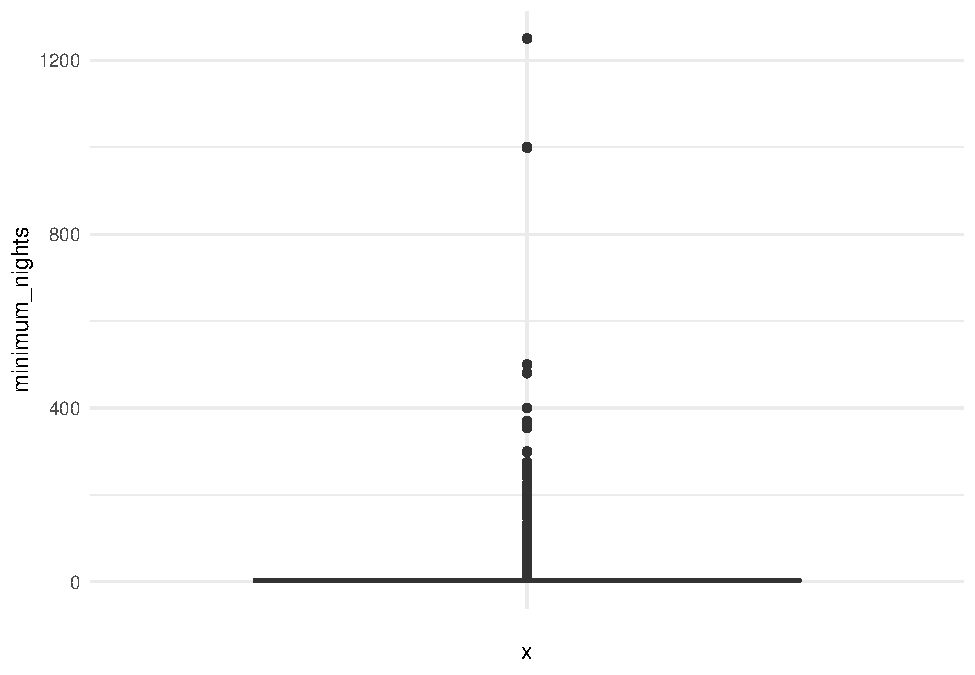
\includegraphics{_main_files/figure-latex/unnamed-chunk-14-4.pdf}

Según la función \texttt{boxplot.stats()\$out} que se basa en el criterio \texttt{IQR}, los valores atípicos para el precio son aquellos mayores que 335 mientras que para el mínimo de noches el umbral está en 12.

\begin{Shaded}
\begin{Highlighting}[]
\FunctionTok{min}\NormalTok{(}\FunctionTok{boxplot.stats}\NormalTok{(df}\SpecialCharTok{$}\NormalTok{price)}\SpecialCharTok{$}\NormalTok{out)}
\end{Highlighting}
\end{Shaded}

\begin{verbatim}
## [1] 335
\end{verbatim}

\begin{Shaded}
\begin{Highlighting}[]
\FunctionTok{min}\NormalTok{(}\FunctionTok{boxplot.stats}\NormalTok{(df}\SpecialCharTok{$}\NormalTok{minimum\_nights)}\SpecialCharTok{$}\NormalTok{out)}
\end{Highlighting}
\end{Shaded}

\begin{verbatim}
## [1] 12
\end{verbatim}

Si revisamos por el criterio de los percentiles, teniendo en cuenta que las observaciones por fuera del intervalo formado por los percentiles 2.5 y 97.5 se consideran posibles valores atípicos, encontramos que para el precio son potenciales datos atípicos aquellos por debajo de 30 y por encima de 799 y en el caso de las noches mínimas, aquellas obervaciones por debajo de 1 y por encima de 30.

\begin{Shaded}
\begin{Highlighting}[]
\FunctionTok{c}\NormalTok{(}\FunctionTok{quantile}\NormalTok{(df}\SpecialCharTok{$}\NormalTok{price, }\FloatTok{0.025}\NormalTok{), }\FunctionTok{quantile}\NormalTok{(df}\SpecialCharTok{$}\NormalTok{price, }\FloatTok{0.975}\NormalTok{))}
\end{Highlighting}
\end{Shaded}

\begin{verbatim}
##  2.5% 97.5% 
##    35   500
\end{verbatim}

\begin{Shaded}
\begin{Highlighting}[]
\FunctionTok{c}\NormalTok{(}\FunctionTok{quantile}\NormalTok{(df}\SpecialCharTok{$}\NormalTok{minimum\_nights, }\FloatTok{0.025}\NormalTok{), }\FunctionTok{quantile}\NormalTok{(df}\SpecialCharTok{$}\NormalTok{minimum\_nights, }\FloatTok{0.975}\NormalTok{))}
\end{Highlighting}
\end{Shaded}

\begin{verbatim}
##  2.5% 97.5% 
##     1    30
\end{verbatim}

Otro método, es el filtro de Hampel que determina que es un dato atípico si el precio está por encima de 244 y las noches minimas superan las 9.

\begin{Shaded}
\begin{Highlighting}[]
\FunctionTok{c}\NormalTok{(}\FunctionTok{median}\NormalTok{(df}\SpecialCharTok{$}\NormalTok{price) }\SpecialCharTok{{-}} \DecValTok{3} \SpecialCharTok{*} \FunctionTok{mad}\NormalTok{(df}\SpecialCharTok{$}\NormalTok{price, }\AttributeTok{constant =} \DecValTok{1}\NormalTok{), }\FunctionTok{median}\NormalTok{(df}\SpecialCharTok{$}\NormalTok{price) }\SpecialCharTok{+} \DecValTok{3} \SpecialCharTok{*} \FunctionTok{mad}\NormalTok{(df}\SpecialCharTok{$}\NormalTok{price, }\AttributeTok{constant =} \DecValTok{1}\NormalTok{))}
\end{Highlighting}
\end{Shaded}

\begin{verbatim}
## [1] -32 244
\end{verbatim}

\begin{Shaded}
\begin{Highlighting}[]
\FunctionTok{c}\NormalTok{(}\FunctionTok{median}\NormalTok{(df}\SpecialCharTok{$}\NormalTok{minimum\_nights) }\SpecialCharTok{{-}} \DecValTok{3} \SpecialCharTok{*} \FunctionTok{mad}\NormalTok{(df}\SpecialCharTok{$}\NormalTok{minimum\_nights, }\AttributeTok{constant =} \DecValTok{1}\NormalTok{), }\FunctionTok{median}\NormalTok{(df}\SpecialCharTok{$}\NormalTok{minimum\_nights) }\SpecialCharTok{+} \DecValTok{3} \SpecialCharTok{*} \FunctionTok{mad}\NormalTok{(df}\SpecialCharTok{$}\NormalTok{minimum\_nights, }\AttributeTok{constant =} \DecValTok{1}\NormalTok{))}
\end{Highlighting}
\end{Shaded}

\begin{verbatim}
## [1] -3  9
\end{verbatim}

Siendo conservadores, eliminaremos la menor cantidad de datos atípicos posibles, que se consiguen al usar el umbral dado por el criterio de los percentiles. Siendo así, estamos eliminando el 2.13\% de nuestros datos, resultando un dataframe con 1.044 registros menos.

\begin{Shaded}
\begin{Highlighting}[]
\FunctionTok{nrow}\NormalTok{(df)}
\end{Highlighting}
\end{Shaded}

\begin{verbatim}
## [1] 48895
\end{verbatim}

\begin{Shaded}
\begin{Highlighting}[]
\FunctionTok{nrow}\NormalTok{(df[df}\SpecialCharTok{$}\NormalTok{price}\SpecialCharTok{\textgreater{}}\DecValTok{335}\NormalTok{, ])}\SpecialCharTok{/}\FunctionTok{nrow}\NormalTok{(df)}\SpecialCharTok{*}\FloatTok{100.00}
\end{Highlighting}
\end{Shaded}

\begin{verbatim}
## [1] 6.06197
\end{verbatim}

\begin{Shaded}
\begin{Highlighting}[]
\FunctionTok{nrow}\NormalTok{(df[df}\SpecialCharTok{$}\NormalTok{price}\SpecialCharTok{\textgreater{}}\DecValTok{500}\NormalTok{, ])}\SpecialCharTok{/}\FunctionTok{nrow}\NormalTok{(df)}\SpecialCharTok{*}\FloatTok{100.00}
\end{Highlighting}
\end{Shaded}

\begin{verbatim}
## [1] 2.135188
\end{verbatim}

\begin{Shaded}
\begin{Highlighting}[]
\FunctionTok{nrow}\NormalTok{(df[df}\SpecialCharTok{$}\NormalTok{price}\SpecialCharTok{\textgreater{}}\DecValTok{244}\NormalTok{, ])}\SpecialCharTok{/}\FunctionTok{nrow}\NormalTok{(df)}\SpecialCharTok{*}\FloatTok{100.00}
\end{Highlighting}
\end{Shaded}

\begin{verbatim}
## [1] 13.26311
\end{verbatim}

Una vez eliminados estos datos atípicos, volveos a extraer las estadísticas de resumen

\begin{Shaded}
\begin{Highlighting}[]
\NormalTok{df\_out }\OtherTok{=}\NormalTok{ df[df}\SpecialCharTok{$}\NormalTok{price}\SpecialCharTok{\textless{}}\DecValTok{500}\NormalTok{, ]}
\FunctionTok{summary}\NormalTok{(df\_out)}
\end{Highlighting}
\end{Shaded}

\begin{verbatim}
##        id              host_id          neighbourhood_group neighbourhood     
##  Min.   :    2539   Min.   :     2438   Length:47660        Length:47660      
##  1st Qu.: 9463850   1st Qu.:  7778878   Class :character    Class :character  
##  Median :19623162   Median : 30567770   Mode  :character    Mode  :character  
##  Mean   :18979918   Mean   : 67134263                                         
##  3rd Qu.:29058184   3rd Qu.:107216950                                         
##  Max.   :36487245   Max.   :274321313                                         
##     latitude       longitude       room_type             price      
##  Min.   :40.50   Min.   :-74.24   Length:47660       Min.   :  0.0  
##  1st Qu.:40.69   1st Qu.:-73.98   Class :character   1st Qu.: 68.0  
##  Median :40.72   Median :-73.96   Mode  :character   Median :100.0  
##  Mean   :40.73   Mean   :-73.95                      Mean   :130.1  
##  3rd Qu.:40.76   3rd Qu.:-73.94                      3rd Qu.:170.0  
##  Max.   :40.91   Max.   :-73.71                      Max.   :499.0  
##  minimum_nights     number_of_reviews reviews_per_month
##  Min.   :   1.000   Min.   :  0.00    Min.   : 0.000   
##  1st Qu.:   1.000   1st Qu.:  1.00    1st Qu.: 0.040   
##  Median :   2.000   Median :  5.00    Median : 0.380   
##  Mean   :   6.978   Mean   : 23.59    Mean   : 1.102   
##  3rd Qu.:   5.000   3rd Qu.: 24.00    3rd Qu.: 1.610   
##  Max.   :1250.000   Max.   :629.00    Max.   :58.500   
##  calculated_host_listings_count availability_365
##  Min.   :  1.000                Min.   :  0     
##  1st Qu.:  1.000                1st Qu.:  0     
##  Median :  1.000                Median : 42     
##  Mean   :  7.096                Mean   :111     
##  3rd Qu.:  2.000                3rd Qu.:221     
##  Max.   :327.000                Max.   :365
\end{verbatim}

\begin{Shaded}
\begin{Highlighting}[]
\FunctionTok{par}\NormalTok{(}\AttributeTok{mfrow =} \FunctionTok{c}\NormalTok{(}\DecValTok{1}\NormalTok{, }\DecValTok{2}\NormalTok{))}

\FunctionTok{ggplot}\NormalTok{(df\_out) }\SpecialCharTok{+}
  \FunctionTok{aes}\NormalTok{(}\AttributeTok{x =}\NormalTok{ price) }\SpecialCharTok{+}
  \FunctionTok{geom\_histogram}\NormalTok{(}\AttributeTok{fill =} \StringTok{"pink"}\NormalTok{) }\SpecialCharTok{+}
  \FunctionTok{theme\_minimal}\NormalTok{()}
\end{Highlighting}
\end{Shaded}

\begin{verbatim}
## `stat_bin()` using `bins = 30`. Pick better value with `binwidth`.
\end{verbatim}

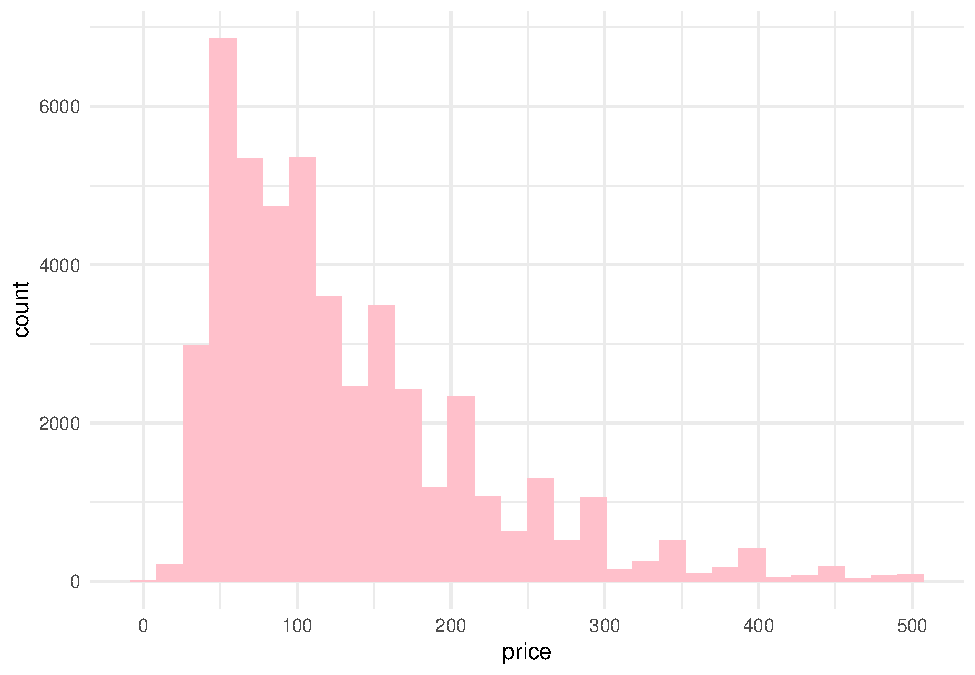
\includegraphics{_main_files/figure-latex/unnamed-chunk-20-1.pdf}

\begin{Shaded}
\begin{Highlighting}[]
\FunctionTok{ggplot}\NormalTok{(df\_out) }\SpecialCharTok{+}
  \FunctionTok{aes}\NormalTok{(}\AttributeTok{x =} \StringTok{""}\NormalTok{, }\AttributeTok{y =}\NormalTok{ price) }\SpecialCharTok{+}
  \FunctionTok{geom\_boxplot}\NormalTok{(}\AttributeTok{fill =} \StringTok{"pink"}\NormalTok{) }\SpecialCharTok{+}
  \FunctionTok{theme\_minimal}\NormalTok{()}
\end{Highlighting}
\end{Shaded}

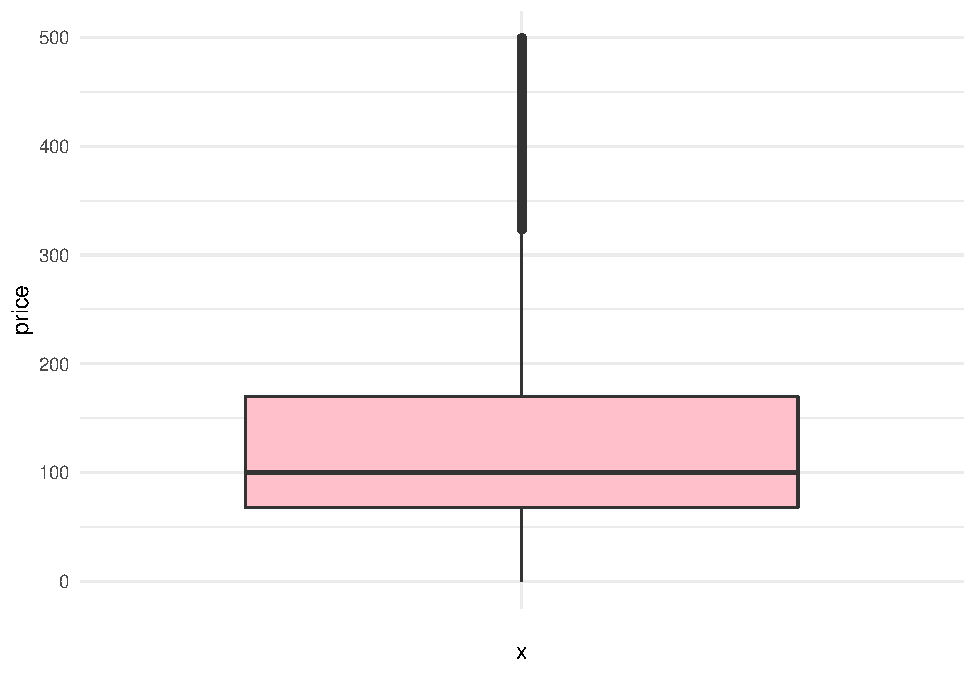
\includegraphics{_main_files/figure-latex/unnamed-chunk-20-2.pdf}

\hypertarget{anuxe1lisis-del-anfitrion}{%
\section*{Análisis del anfitrion}\label{anuxe1lisis-del-anfitrion}}
\addcontentsline{toc}{section}{Análisis del anfitrion}

A través de la función de agrupación \texttt{group\_by}, podemos obtener los anfitriones con más alojamientos disponibles, encontrando que el mayor tiene 272 lo que no es consistente con el máximo valor encontrado en la columna \texttt{calculated\_host\_listings\_count} debido a la eliminación de datos atípicos realizados anteriormente, es por esto, que esta columna, se eliminará del dataframe.

\begin{Shaded}
\begin{Highlighting}[]
\NormalTok{df\_out }\SpecialCharTok{\%\textgreater{}\%}
  \FunctionTok{group\_by}\NormalTok{(host\_id) }\SpecialCharTok{\%\textgreater{}\%}
  \FunctionTok{summarise}\NormalTok{(}\AttributeTok{n =} \FunctionTok{n}\NormalTok{()) }\SpecialCharTok{\%\textgreater{}\%}
  \FunctionTok{arrange}\NormalTok{(}\FunctionTok{desc}\NormalTok{(n)) }\SpecialCharTok{\%\textgreater{}\%}
  \FunctionTok{head}\NormalTok{(}\DecValTok{5}\NormalTok{) }\OtherTok{{-}\textgreater{}}\NormalTok{ top\_hostid}
\end{Highlighting}
\end{Shaded}

\begin{verbatim}
## `summarise()` ungrouping output (override with `.groups` argument)
\end{verbatim}

\begin{Shaded}
\begin{Highlighting}[]
\FunctionTok{ggplot}\NormalTok{(}\AttributeTok{data=}\NormalTok{ top\_hostid, }\FunctionTok{aes}\NormalTok{(}\AttributeTok{x =} \FunctionTok{factor}\NormalTok{(host\_id), }\AttributeTok{y=}\NormalTok{n)) }\SpecialCharTok{+}
  \FunctionTok{geom\_bar}\NormalTok{(}\AttributeTok{stat=}\StringTok{"identity"}\NormalTok{, }\AttributeTok{fill =} \StringTok{"blue"}\NormalTok{) }\SpecialCharTok{+}
  \FunctionTok{xlab}\NormalTok{(}\StringTok{"Host\_Id"}\NormalTok{) }\SpecialCharTok{+} \FunctionTok{ylab}\NormalTok{(}\StringTok{"Cant. alojamientos"}\NormalTok{) }\SpecialCharTok{+}
  \FunctionTok{ggtitle}\NormalTok{(}\StringTok{"Top 5 de los anfitriones con más alojamientos"}\NormalTok{)}
\end{Highlighting}
\end{Shaded}

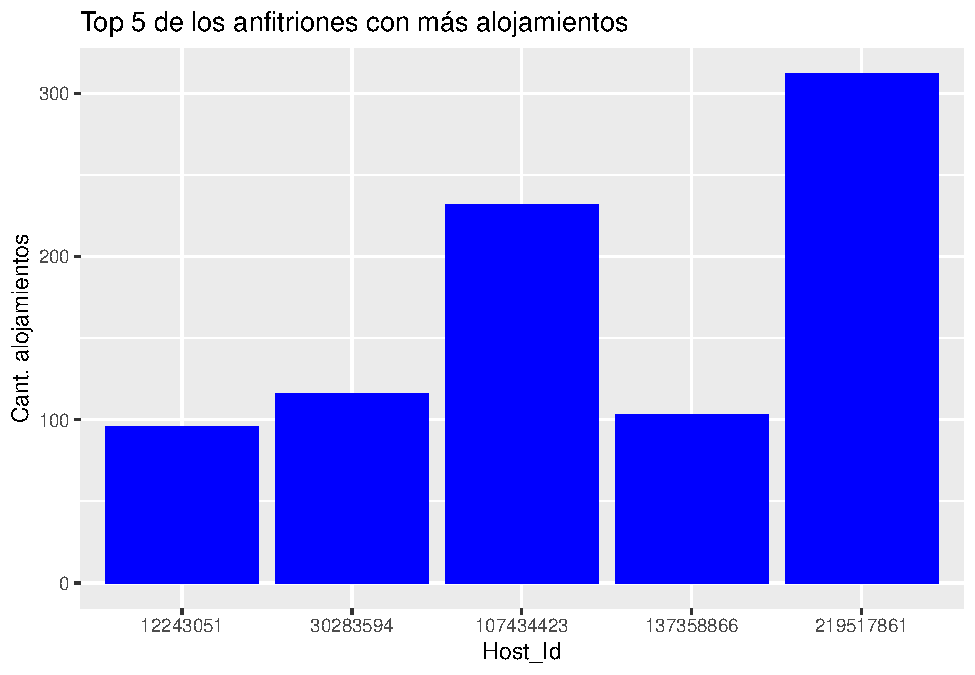
\includegraphics{_main_files/figure-latex/unnamed-chunk-21-1.pdf}

\begin{Shaded}
\begin{Highlighting}[]
\NormalTok{borrar }\OtherTok{=} \FunctionTok{c}\NormalTok{(}\StringTok{"calculated\_host\_listings\_count"}\NormalTok{)}
\NormalTok{df\_out }\OtherTok{=}\NormalTok{ df\_out[, }\SpecialCharTok{!}\NormalTok{(}\FunctionTok{names}\NormalTok{(df\_out) }\SpecialCharTok{\%in\%}\NormalTok{ borrar)]}
\end{Highlighting}
\end{Shaded}

Ahora, revisemos la distribución de alojamientos por grupos de vecindarios.

\begin{Shaded}
\begin{Highlighting}[]
\NormalTok{df\_host }\OtherTok{=} \FunctionTok{filter}\NormalTok{(df\_out, host\_id }\SpecialCharTok{\%in\%}\NormalTok{ top\_hostid}\SpecialCharTok{$}\NormalTok{host\_id)}

\NormalTok{df\_host}\SpecialCharTok{\%\textgreater{}\%}
  \FunctionTok{group\_by}\NormalTok{(host\_id, neighbourhood\_group) }\SpecialCharTok{\%\textgreater{}\%}
  \FunctionTok{summarise}\NormalTok{(}\AttributeTok{n =} \FunctionTok{n}\NormalTok{()) }\SpecialCharTok{\%\textgreater{}\%}
  \FunctionTok{ggplot}\NormalTok{(}\FunctionTok{aes}\NormalTok{(}\AttributeTok{x=}\FunctionTok{factor}\NormalTok{(host\_id), }\AttributeTok{y=}\NormalTok{n, }\AttributeTok{fill=}\FunctionTok{factor}\NormalTok{(neighbourhood\_group))) }\SpecialCharTok{+} 
  \FunctionTok{geom\_bar}\NormalTok{(}\AttributeTok{stat=}\StringTok{"identity"}\NormalTok{, }\AttributeTok{position=}\StringTok{"dodge"}\NormalTok{)}\SpecialCharTok{+}
  \FunctionTok{xlab}\NormalTok{(}\StringTok{"Host\_id"}\NormalTok{) }\SpecialCharTok{+} \FunctionTok{ylab}\NormalTok{(}\StringTok{"Cant. Alojamientos"}\NormalTok{) }\SpecialCharTok{+}
  \FunctionTok{ggtitle}\NormalTok{(}\StringTok{"Top 5 de anfitriones con más alojamientos distribuidos por grupo vecindario"}\NormalTok{)}\SpecialCharTok{+}
  \FunctionTok{theme}\NormalTok{()}
\end{Highlighting}
\end{Shaded}

\begin{verbatim}
## `summarise()` regrouping output by 'host_id' (override with `.groups` argument)
\end{verbatim}

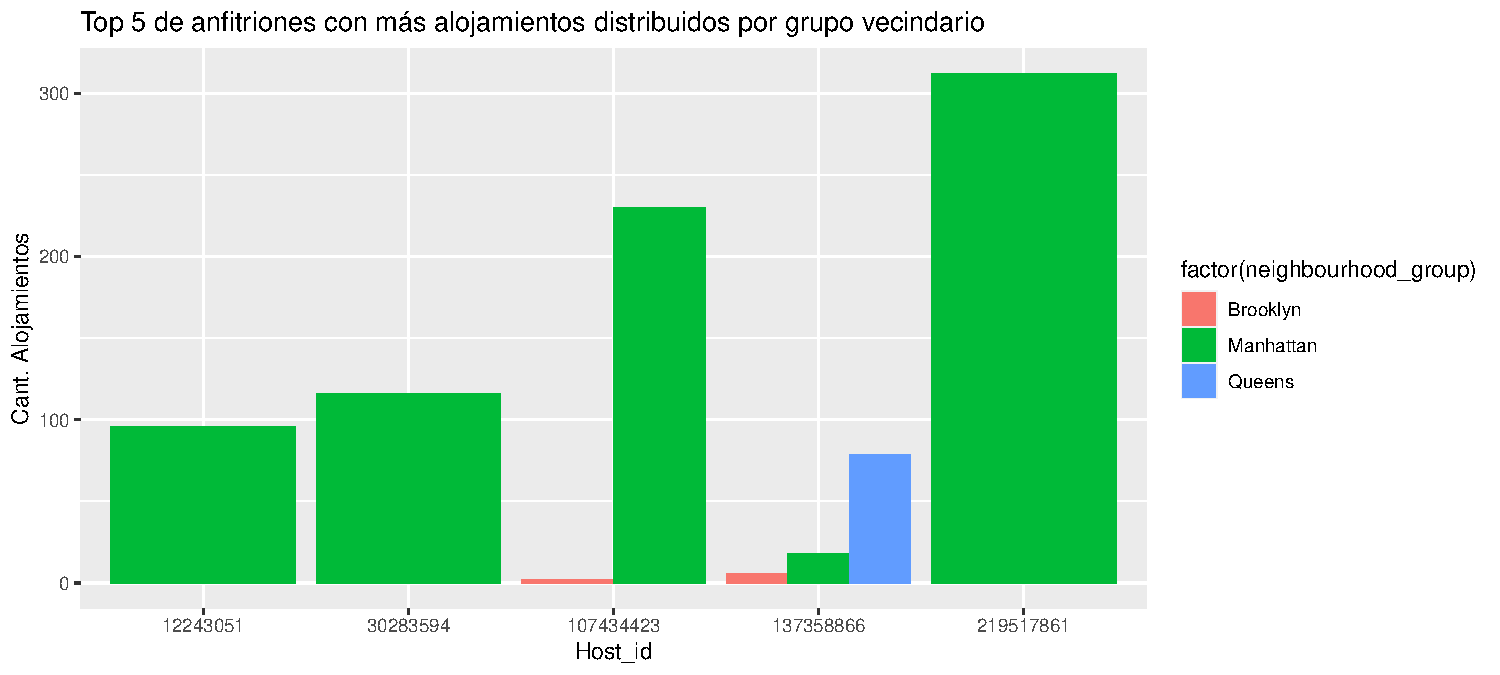
\includegraphics{_main_files/figure-latex/unnamed-chunk-22-1.pdf}

A pesar, que los grupos de vecindarios disponibles coresponden a Brooklyn, Manhattan, Qeens, Staten Island y Bronx, vemos que los anfitriones con más alojamientos no tienen disponibilidad en Staten Island y Bronx y exceptuando el host 137358866, la mayoría de estos alojamientos se encuentran en Manhattan y solo dos de estos cinco tienenalojamientos en Brooklyn.

Si revisamos la distribución de los precios de estos cinco anfitriones, atraves, de un \texttt{boxplot}, tenemos que el anfitrion 107434423 tiene el mayor precio promedio y el anfitrion 137358866 tiene todos sus alojamnientos en precios similares y más bajos en comparación con los otros.

\begin{Shaded}
\begin{Highlighting}[]
\NormalTok{df\_host}\SpecialCharTok{\%\textgreater{}\%}
  \FunctionTok{ggplot}\NormalTok{(}\FunctionTok{aes}\NormalTok{(}\AttributeTok{x=}\FunctionTok{factor}\NormalTok{(host\_id), }\AttributeTok{y=}\NormalTok{price)) }\SpecialCharTok{+} 
  \FunctionTok{geom\_boxplot}\NormalTok{(}\AttributeTok{fill =} \StringTok{"pink"}\NormalTok{)}\SpecialCharTok{+}
  \FunctionTok{xlab}\NormalTok{(}\StringTok{"Host\_Id"}\NormalTok{) }\SpecialCharTok{+} \FunctionTok{ylab}\NormalTok{(}\StringTok{"Precio"}\NormalTok{) }\SpecialCharTok{+}
  \FunctionTok{ggtitle}\NormalTok{(}\StringTok{"Distribución de precios para los 5 anfitriones con más alojamientos"}\NormalTok{)}
\end{Highlighting}
\end{Shaded}

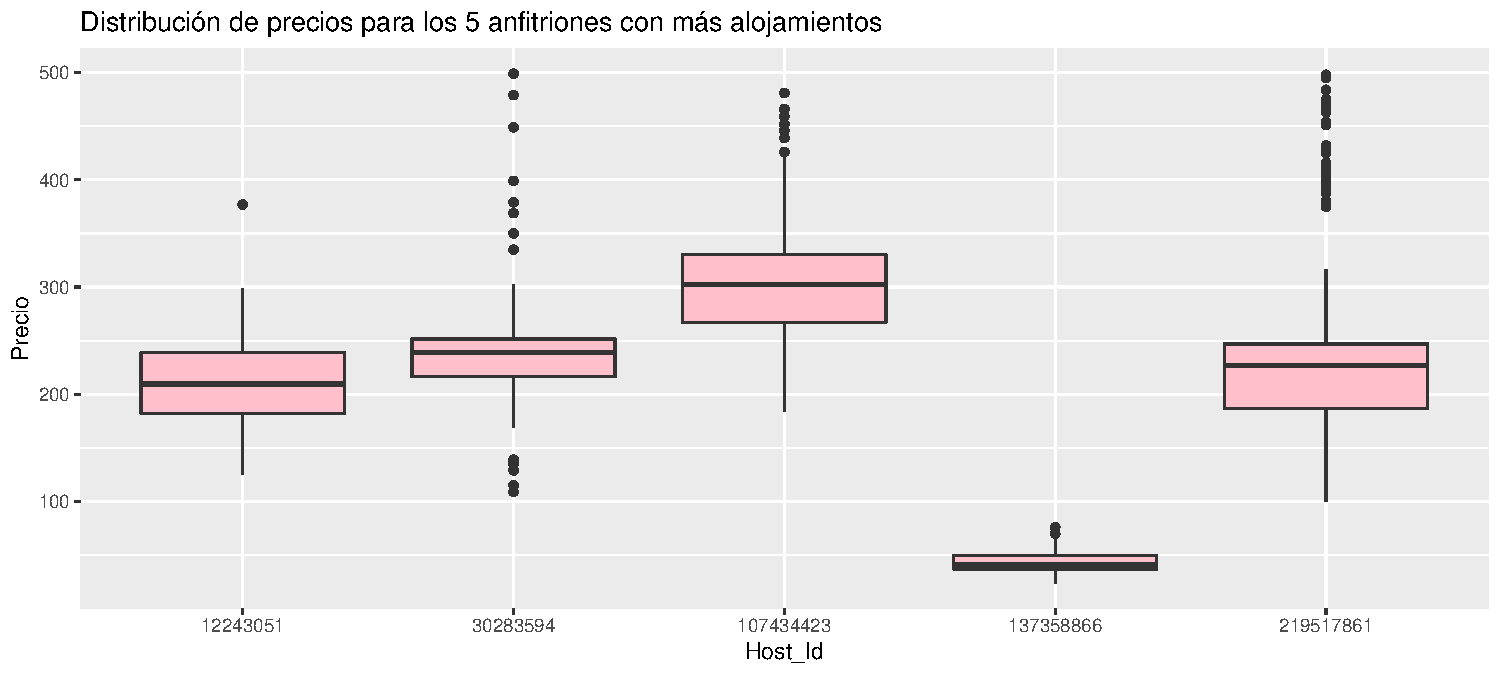
\includegraphics{_main_files/figure-latex/unnamed-chunk-23-1.pdf}

\begin{Shaded}
\begin{Highlighting}[]
  \FunctionTok{theme}\NormalTok{()}
\end{Highlighting}
\end{Shaded}

\begin{verbatim}
##  Named list()
##  - attr(*, "class")= chr [1:2] "theme" "gg"
##  - attr(*, "complete")= logi FALSE
##  - attr(*, "validate")= logi TRUE
\end{verbatim}

\hypertarget{anuxe1lisis-de-los-precios}{%
\section*{Análisis de los precios}\label{anuxe1lisis-de-los-precios}}
\addcontentsline{toc}{section}{Análisis de los precios}

Si ahora revisamos los precios, vemos que el mayor precio promedio por noche está en la zona de Manhattan para los tres tipos de alojamiento, adicionalmente y como era de esperarse, es más costoso un alojamiento completo, seguido de una habitación privada y por útimo una habitación compartida, aunque no hay una gran diferencia entre los valores promedios de las habitaciones. Este patrón se mantiene igual, independiente del grupo de vecindario al que pertenezca.

\begin{Shaded}
\begin{Highlighting}[]
\NormalTok{df\_out }\SpecialCharTok{\%\textgreater{}\%}
  \FunctionTok{group\_by}\NormalTok{(neighbourhood\_group, room\_type)}\SpecialCharTok{\%\textgreater{}\%}
  \FunctionTok{summarise}\NormalTok{(}\AttributeTok{m =} \FunctionTok{mean}\NormalTok{(price)) }\OtherTok{{-}\textgreater{}}\NormalTok{ group\_type}
\end{Highlighting}
\end{Shaded}

\begin{verbatim}
## `summarise()` regrouping output by 'neighbourhood_group' (override with `.groups` argument)
\end{verbatim}

\begin{Shaded}
\begin{Highlighting}[]
\NormalTok{group\_type}\SpecialCharTok{\%\textgreater{}\%}
  \FunctionTok{ggplot}\NormalTok{(}\FunctionTok{aes}\NormalTok{(}\AttributeTok{x=}\NormalTok{room\_type, }\AttributeTok{y=}\NormalTok{m, }\AttributeTok{fill=}\NormalTok{room\_type)) }\SpecialCharTok{+} 
  \FunctionTok{geom\_bar}\NormalTok{(}\AttributeTok{stat=}\StringTok{"identity"}\NormalTok{)}\SpecialCharTok{+}
  \FunctionTok{facet\_wrap}\NormalTok{(}\SpecialCharTok{\textasciitilde{}}\NormalTok{neighbourhood\_group)}\SpecialCharTok{+}
  \FunctionTok{xlab}\NormalTok{(}\StringTok{"Grupo Vecindario"}\NormalTok{) }\SpecialCharTok{+} \FunctionTok{ylab}\NormalTok{(}\StringTok{"Precio Medio"}\NormalTok{) }\SpecialCharTok{+}
  \FunctionTok{ggtitle}\NormalTok{(}\StringTok{"Precio promedio por grupo de vecindario y tipo de alojamiento"}\NormalTok{)}\SpecialCharTok{+}
  \FunctionTok{theme}\NormalTok{(}\AttributeTok{axis.text.x=}\FunctionTok{element\_blank}\NormalTok{())}
\end{Highlighting}
\end{Shaded}

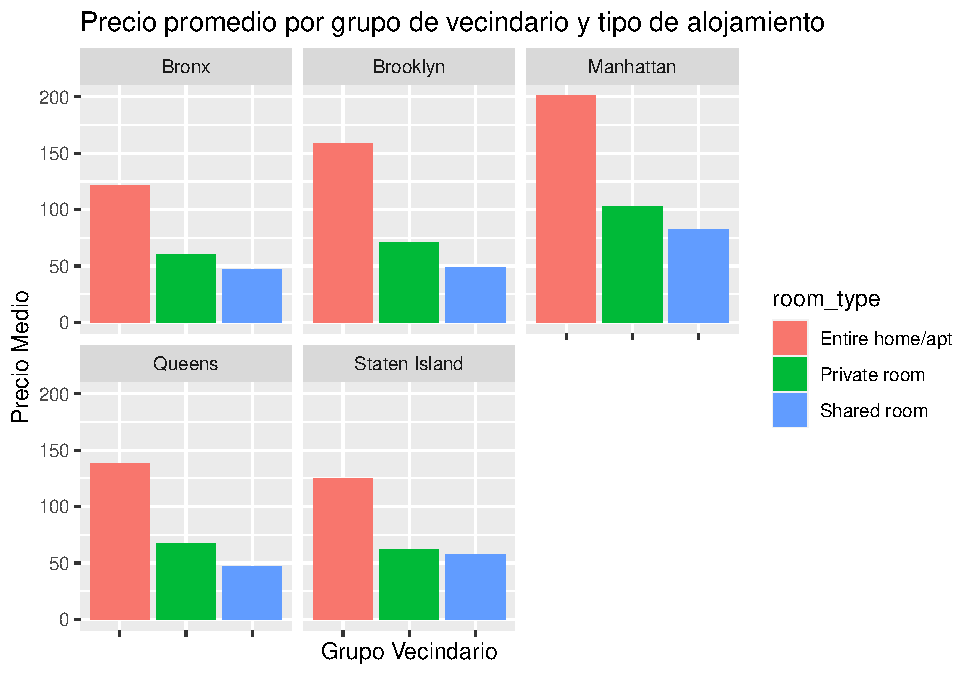
\includegraphics{_main_files/figure-latex/unnamed-chunk-24-1.pdf}

El grupo de vecindario con el precio promedio más alto es Manhattan y en este grupo se manejan el mayor rango de precios. Los precios para Queen y Staten Island tienen distribuciones similares.

\begin{Shaded}
\begin{Highlighting}[]
\FunctionTok{ggplot}\NormalTok{(}\AttributeTok{data=}\NormalTok{df\_out, }\AttributeTok{mapping =} \FunctionTok{aes}\NormalTok{(}\AttributeTok{x=}\NormalTok{neighbourhood\_group, }\AttributeTok{y=}\NormalTok{price)) }\SpecialCharTok{+}
  \FunctionTok{geom\_violin}\NormalTok{()}\SpecialCharTok{+}
  \FunctionTok{geom\_boxplot}\NormalTok{(}\AttributeTok{width=}\FloatTok{0.2}\NormalTok{)}
\end{Highlighting}
\end{Shaded}

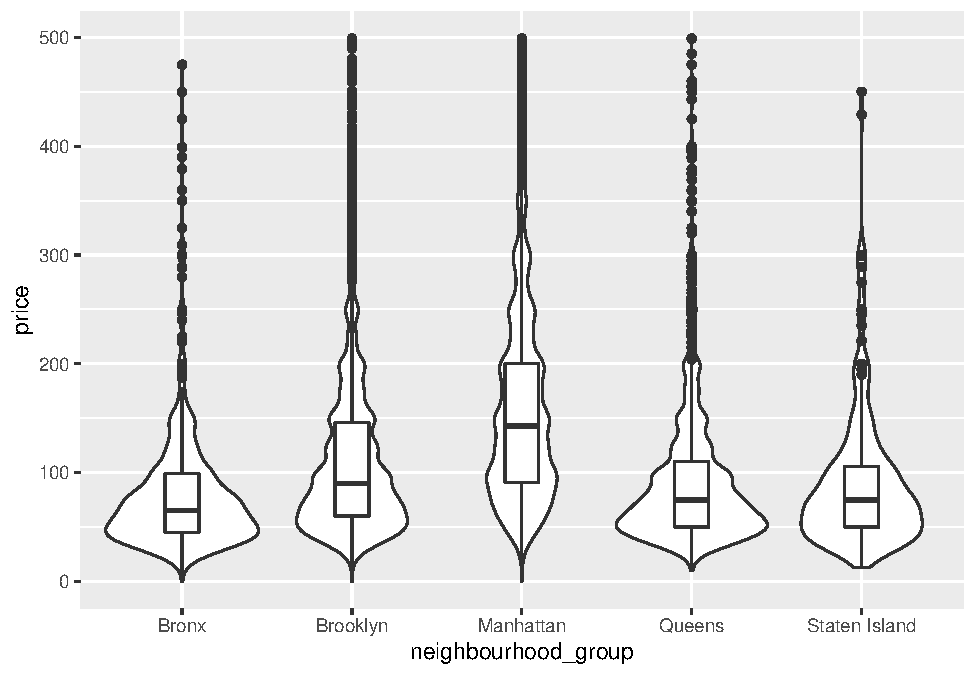
\includegraphics{_main_files/figure-latex/unnamed-chunk-25-1.pdf}

Si agrupamos por tipo de alojamiento, vemos que los valores por habitaión compartida en Staten Island presentan una distribución distintas a las demás con un rango mayor y un sesgo hacia la izquierda. En cuanto a las habitaciones privadas tenemos una alta concentración de valores atípicos. En los alojamientos completos por grupo el precio es consistente, sin muchos valores atípicos.

\begin{Shaded}
\begin{Highlighting}[]
\FunctionTok{ggplot}\NormalTok{(}\AttributeTok{data=}\NormalTok{df\_out, }\AttributeTok{mapping =} \FunctionTok{aes}\NormalTok{(}\AttributeTok{x=}\NormalTok{neighbourhood\_group, }\AttributeTok{y=}\NormalTok{price)) }\SpecialCharTok{+}
  \FunctionTok{geom\_violin}\NormalTok{()}\SpecialCharTok{+}
  \FunctionTok{geom\_boxplot}\NormalTok{(}\AttributeTok{width=}\FloatTok{0.2}\NormalTok{)}\SpecialCharTok{+}
  \FunctionTok{facet\_wrap}\NormalTok{(}\SpecialCharTok{\textasciitilde{}}\NormalTok{room\_type)}
\end{Highlighting}
\end{Shaded}

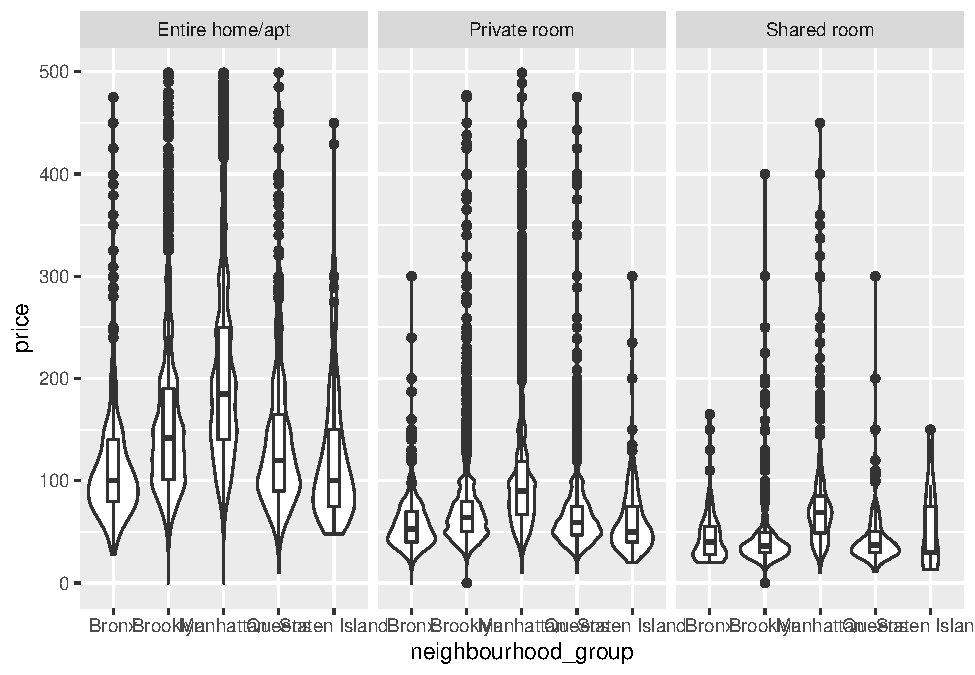
\includegraphics{_main_files/figure-latex/unnamed-chunk-26-1.pdf}

\hypertarget{visualziaciuxf3n-en-mapas}{%
\section*{Visualziación en mapas}\label{visualziaciuxf3n-en-mapas}}
\addcontentsline{toc}{section}{Visualziación en mapas}

Para los datos de interés, contamos con la ubicación (latitud, longitud) de los alojamientos en Nueva York. Revisaremos la distribución de estos en un mapa, através de la función \texttt{gg\_map}, ubicándonos precisamente en Nueva York, encontrando que la menor cantidad de alojamientos se encuentra en ``Staten Island''

\begin{Shaded}
\begin{Highlighting}[]
\NormalTok{myLocation }\OtherTok{\textless{}{-}} \StringTok{"Nueva York"}

\NormalTok{myMap }\OtherTok{\textless{}{-}} \FunctionTok{get\_map}\NormalTok{(}\AttributeTok{location =}\NormalTok{ myLocation, }\AttributeTok{zoom =} \DecValTok{10}\NormalTok{)}
\end{Highlighting}
\end{Shaded}

\begin{verbatim}
## Source : https://maps.googleapis.com/maps/api/staticmap?center=Nueva%20York&zoom=10&size=640x640&scale=2&maptype=terrain&language=en-EN&key=xxx
\end{verbatim}

\begin{verbatim}
## Source : https://maps.googleapis.com/maps/api/geocode/json?address=Nueva+York&key=xxx
\end{verbatim}

\begin{Shaded}
\begin{Highlighting}[]
\FunctionTok{ggmap}\NormalTok{(myMap) }\SpecialCharTok{+} \FunctionTok{geom\_point}\NormalTok{(}\AttributeTok{data=}\NormalTok{df\_out, }\FunctionTok{aes}\NormalTok{(}\AttributeTok{x =}\NormalTok{ longitude, }\AttributeTok{y =}\NormalTok{ latitude, }\AttributeTok{colour=}\NormalTok{ neighbourhood\_group))}
\end{Highlighting}
\end{Shaded}

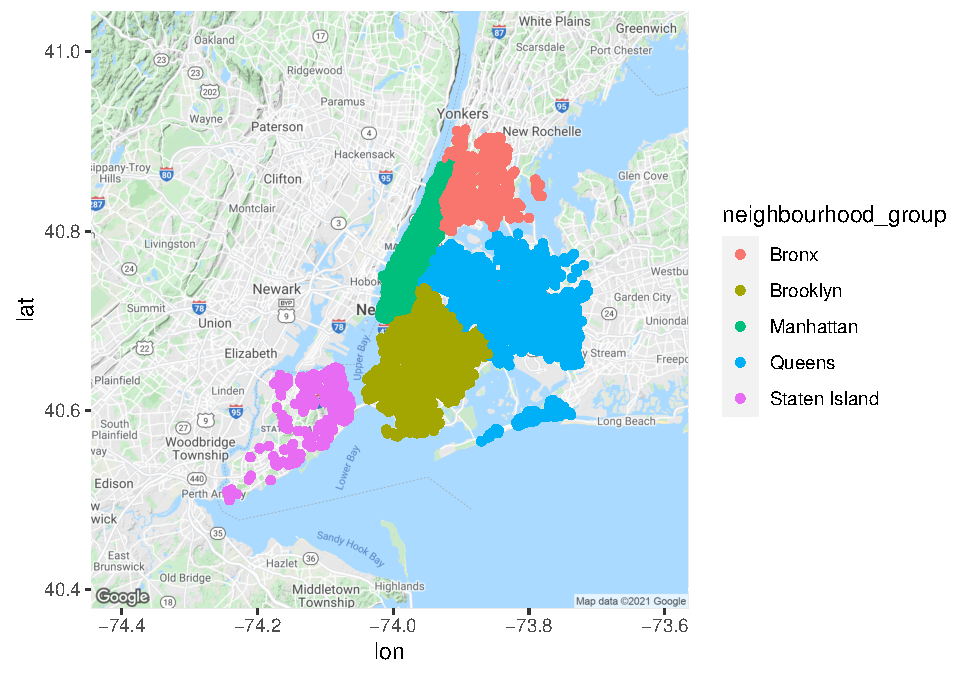
\includegraphics{_main_files/figure-latex/unnamed-chunk-27-1.pdf}

En Bronx, hay pocos precios altos en los alojamientos y los que existen se encuebntran a los alrededores de la localidad. Si nos enfocamos en Manhattan, vemos que hay una clara división en los precios, los menores se encuentran al norte y los mayores al sur.

En general hay pocos alojamientos con precios altos en comparación con los de precios bajos.

\begin{Shaded}
\begin{Highlighting}[]
\FunctionTok{ggmap}\NormalTok{(myMap) }\SpecialCharTok{+} 
  \FunctionTok{geom\_point}\NormalTok{(}\AttributeTok{data=}\NormalTok{df\_out, }\FunctionTok{aes}\NormalTok{(}\AttributeTok{x =}\NormalTok{ longitude, }\AttributeTok{y =}\NormalTok{ latitude, }\AttributeTok{colour=}\NormalTok{ price))}\SpecialCharTok{+}
  \FunctionTok{scale\_color\_gradientn}\NormalTok{(}\AttributeTok{colours =} \FunctionTok{rainbow}\NormalTok{(}\DecValTok{5}\NormalTok{))}\SpecialCharTok{+}
  \FunctionTok{facet\_wrap}\NormalTok{(}\SpecialCharTok{\textasciitilde{}}\NormalTok{neighbourhood\_group)}
\end{Highlighting}
\end{Shaded}

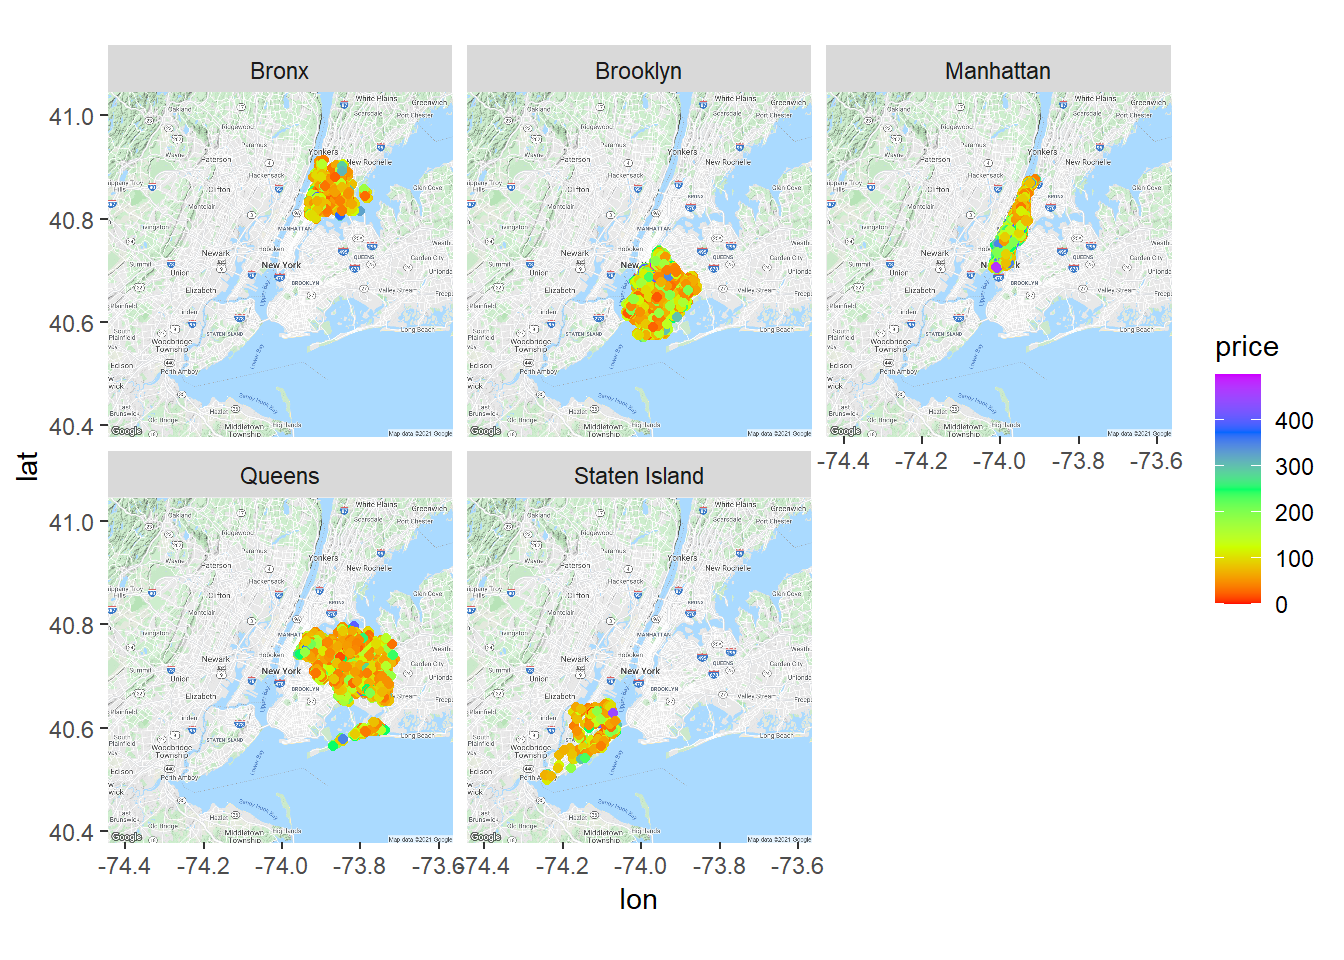
\includegraphics{_main_files/figure-latex/unnamed-chunk-28-1.pdf}

  \bibliography{book.bib,packages.bib}

\end{document}
